\chapter{Theory: advanced structural results}
\label{chap.theorystructure}



Within this chapter, we introduce innovative theoretical findings related to the process of convexification or relaxation of structured sets. These findings have been developed to address practical challenges encountered throughout this thesis and will serve as the foundation for the development of cutting-edge algorithms for various problems. These results can be regarded as advanced concepts building upon the submodularity and intersection cut framework introduced in \Cref{chap.basic}.

\section{$\cS$-free sets for structured sets}
\label{sec.advanced}

In this section, we introduce advanced results concerning the intersection cut framework. We have demonstrated that the intersection cuts relies on the concept of $\cS$-free sets, which in turn, depend on the specific problem structure. The set $\cS$ under consideration encompasses sets originating from NLP and those arising in submodular optimization.


\subsection{Maximal $\cS$-free sets for lifted sets}
\label{sec.lift}
We  consider  the extended formulation \eqref{minlp3} of a general NLP problem and focus on the associated lifted set $\cSl$ in \eqref{eq.lift}.  We show a lifting result on the construction of maximal $\cSl$-free sets.



Let $z\deq(x,y)$ denote the vector variable in the extended formulation \eqref{minlp3}, with its index set being $[n+k]$. Consequently, we have $z_{[n]} = x$ and $z_{[n+1:n+k]} = y$. Consider a closed subset $\cX$ of the domain $\bigcap_{i \in [k]} \dom(g_i)$ for $x$, and let $\cY$ be a closed subset of the domain $\bigtimes_{i \in [k]} \rang(g_i)$ for $y$. The ground set $\cG$, where the variables actually vary, can be set as $\cX \times \cY$. Consequently, the lifted set $\cSl$ in \eqref{eq.lift} admits the form $\{(x,y) \in \cG: y = g(x)\}$.

Given that each $g_i(x)$ (for $i\in[k]$) may only depend on a subset of  variables indexed by $J_i \subseteq [n]$, we can express $g_i(x)$ as a lower order function $g'_i(x_{J_i})$ defined over $\bR^{|J_i|}$. Let $I_i \deq J_i \cup \{i + n\}$. As above, we consider a closed subset $\cX^i$ of $\dom(g'_i)$ and $\cY^i$ of $\rang(g'_i)$. Consequently, the graph, epigraph, and hypograph of $g'_i$ reside within sets $\cG^i \deq \cX^i \times \cY^i$, \eg $\epi(g'_i)=\{(x_{J_i}, y_i) \in \cG^i: g'_i(x_{J_i}) \le y_i\}$.

We refer to $\cX,\cY, \{\cX^i, \cY^i\}_{i \in [k]}$ as the \emph{underlying sets} of the lifted set $\cSl$. The sets are said to be \emph{1d-convex decomposable} by a collection $\{\cD_j \}_{j \in [n+k]}$ of closed  convex sets in $\bR$, if  $\cX= \bigtimes_{j \in [n]}\cD_j, \cY= \bigtimes_{j \in [n+1:n+k]}\cD_j$, and, for all $i \in [k]$, $\cX^i = \bigtimes_{j \in J_i}\cD_j, \cY^i = \cD_{n+i}$. This decomposability condition restricts the domains to Cartesian products of real lines, intervals, or half rays, thereby excluding complicated domain structures.

The decomposability condition allows for the analysis of sets involving fewer variables. Constructing $\epi(g'_i)$-free sets and $\hyp(g'_i)$-free sets is generally easier than constructing $\cSl$-free sets.  We show that every maximal $\epi(g'_i)$-free or $\hyp(g'_i)$-free set can be lifted into a  maximal $\cSl$-free set.

\begin{theorem}
\label{thm.decomp}
Suppose the underlying sets of $\cSl$ are 1d-convex decomposable and $g$ is continuous. For some $i \in [k]$, let $\cC$ be a maximal $\epi(g'_i)$-free set or a maximal $\hyp(g'_i)$-free set in $\cG^i$. Then $\bar{\cC}\deq \cC \times \bR^{|I^c_i|}$ ($I^c_i = [n+k] \setminus I_i$) is a maximal $\cSl$-free set in $\cG$.
\end{theorem}
\begin{proof}
It suffices to consider the case that $\cC$ is a maximal $\epi(g'_i)$-free set in $\cG^i$. W.l.o.g., we can assume that $\cC,  \cG^i$ are full-dimensional in $\bR^{|I_i|}$. Since $\epi(g'_i)$ includes $\gr(g'_i)$, $\cC$, as an $\epi(g'_i)$-free set,  is also $\gr(g'_i)$-free. First, we prove that  $\cC$ is a maximal $\gr(g'_i)$-free set in $\cG^i$. Assume, to aim at a contradiction, that $\cC'$ is a $\gr(g'_i)$-free set that $\cC \cap \cG^i \subsetneq \cC' \cap \cG^i$.  Suppose that $\epi(g'_i)  \cap \inter(\cC' \cap \cG^i)$ is not empty and contains $(x'_{J_i}, y'_i)$.     As $\cC$ is  $\epi(g'_i)$-free, there exists a point $(x_{J_i}, y_i) \in \inter(\cC \cap \cG^i) \subseteq \inter(\cC' \cap \cG^i)$ such that $(x_{J_i}, y_i) \in \hyp(g'_i)$.  It follows from the continuity of $g'_i$  that there exists a point $(x^\ast_{J_i}, y^\ast_i) \in \gr(g'_i)$ in the line segment joining $(x_{J_i}, y_i)$ and $(x'_{J_i}, y'_i) $. As $\inter(\cC' \cap \cG^i)$ is convex,  we have that $(x^\ast_{J_i}, y^\ast_i) \in \inter(\cC' \cap \cG^i)$, which leads to a contradiction to $\gr(g'_i)$-freeness of $\cC'$. Therefore, $\epi(g'_i)  \cap \inter(\cC' \cap \cG^i)$ must be empty, so $\cC' \cap \cG^i  \subseteq \hyp(g'_i)$. This means that $\cC'$ is also $\epi(g'_i)$-free. However, note that  $\cC \cap \cG^i \subsetneq \cC' \cap \cG^i$, this contradicts with the fact that $\cC$ is a maximal $\epi(g'_i)$-free set in $\cG^i$. Therefore, $\cC$  is a maximal $\gr(g'_i)$-free set in $\cG^i$. Secondly, we  prove that $\bar{\cC}$ is a maximal $\cSl$-free set in $\cG$.
Assume, to aim at a contradiction, that there exists an $\cSl$-free set $\bar{\cD}$ in $\cG$ such that $ \bar{\cC} \cap \cG \subsetneq \bar{\cD} \cap \cG$. We look at their orthogonal projections on  $\bR^{|I_i|}$. It follows from the decomposability  that $\cC \cap \cG^i = \cC \cap \proj_{\bR^{|I_i|}} (\cG) = \proj_{\bR^{|I_i|}}(\bar{\cC} \cap \cG) \subseteq \proj_{\bR^{|I_i|}}(\bar{\cD} \cap \cG)$. Denote $\cD \deq \cl(\proj_{\bR^{|I_i|}}(\bar{\cD} \cap \cG))$, which is a closed convex set in $\cG^i$. Since $\bar{\cC}= \cC \times \bR^{|I^c_i|}$, $\cD$  must strictly include $\cC \cap \cG^i$. Note that $\cD$ is $\gr(g'_i)$-free. Since $\cC$ is a maximal $\gr(g'_i)$-free set in $\cG^i$, this implies that $\cC \cap \cG^i = \cD$, which leads to a contradiction.
\end{proof}

 For any $i\in[k]$, we call the operation $\cC \times \bR^{|I^c_i|}$ the \emph{orthogonal lifting} of $\cC$ w.r.t. $g_i$. A similar lifting result for integer programming is provided by Lemma 4.1 of \cite{conforti2011}: given $\cS \deq \bZ^{n} \times \bR^{h}$, any maximal lattice-free set (\ie $\bZ^n$-free set) can be transformed into a maximal $\cS$-free set through orthogonal lifting. Therefore, \Cref{thm.decomp} serves as the NLP counterpart to that lemma (whose proof is also similar). This theorem allows us to focus on low-dimensional projections of the lifted set.

 We will show in \Cref{cor.maxsig} that the signomial lift satisfies the prerequisites of  \Cref{thm.decomp}.
The following example illustrates the application of \Cref{thm.decomp}.

\begin{example}
 Consider a lifted set $\cSl$ defined as $$\{(x_1,x_2,x_3,x_4, y_1,y_2, y_3): y_1= \exp(x_1 - x_2 /x_3),  y_2 = \log(x_1), y_3 = \sin(x_1 / x_4)\}.$$

One can verify that the 1d-convex decomposable condition holds for $\cD_1 = \bR_+$,  $\cD_j = \bR$ (for $j \in [2:7]$). Then $\cG\deq \bR^1_+ \times \bR^6$.  We use $\log(x_1)$ to construct a $\cSl$-free set. A maximal $\cSl$-free set can be $\{(x_1,x_2,x_3,x_4, y_1,y_2, y_3) \in \cG:  y_2 \le \log(x_1)\}$. Since $\log(x_1)$ is defined over positive  reals, this example gives a reason to restrict maximality over $\cG$.
\end{example}




\subsection{Maximal $\cS$-free for DCC constraints}

We provide sufficient conditions for the maximality of $\cS$-free sets for two general classes of non-convex sets $\cS$. To begin with, we review some fundamental results from convex analysis. Our subsequent presentation relies on the use of support functions of convex sets. The properties of support functions can be summarized as follows.


\begin{lemma}[Chapter C of \cite{hiriart2004fundamentals}]
\label{lem.supconv}
 For  a full-dimensional closed convex set  \(\cC \subsetneq \bR^p\), let \(\sigma_{\cC}: \bR^p \to \bR, \lambda \mapsto \sup_{z \in \cC}{\lambda}\cdot z\) be the support function of \(\cC\). Then: (i) \label{lem.supconv2} \(\cC = \{z \in \bR^p: {\lambda}\cdot z\le \sigma_{\cC}({\lambda}), \forall {\lambda} \in \dom(\sigma_{\cC}) \}\), (ii)  \(\inter(\cC) = \{z \in \bR^p:{\lambda}\cdot z <\sigma_{\cC}({\lambda}),  \forall {\lambda} \in  \dom(\sigma_{\cC})  \smallsetminus\{0\} \}\), (iii)
	$\sigma_{\cC}(\rho \lambda) = \rho \sigma_{\cC}(\lambda)$ for any $\rho > 0$. Moreover, for any closed convex set \(\cC'\) including $\cC$,   $\sigma_{\cC} \le \sigma_{\cC'}$.
\end{lemma}

 A valid inequality $a \cdot z \le b$ of $\cC$ is  called a \emph{supported valid inequality}, if there exists a \emph{supporting point} $z' \in \bd(C)$ such that \(a \cdot z' =  b\).  Geometrically, a closed convex set is the intersection of half-spaces associated with supported valid inequalities.


 \begin{observation}
  It follows from \Cref{lem.supconv} that every supported valid inequality of $\cC$ must admit the form $\lambda \cdot z\le \sigma_{\cC}(\lambda)$  for some $\lambda \in \dom(\sigma_{\cC})$, where the supremum  $\sigma_{\cC}(\lambda)$ is attained at its supporting points.
 \end{observation}

An inequality of the form $\lambda \cdot z \leq \sigma_{\cC}(\lambda)$, for $\lambda \in \dom(\sigma_{\cC})$, is referred to as an \emph{exposed valid inequality}, if there exists an \emph{exposing point} $z' \in \bd(C)$ such that $\lambda \cdot z' = \sigma_{\cC}(\lambda)$ and  for all \({\lambda'} \in \dom(\sigma_\cC) \smallsetminus\{{\rho\lambda}\}_{\rho > 0}\), \({\lambda'}\cdot z' < \sigma_{\cC}(\lambda')\).
 
  \begin{observation}
  \label{obs.1}
An exposed valid inequality must be a supported valid inequality. Conversely, a supported valid inequality  is  an exposed valid inequality, if manifold $\bd(\cC)$ is smooth at its supporting point.  For example, $\cC_1\deq\{(x,y) \in \bR^2: y = x^2\}$ is a smooth manifold, so every supported valid inequality of $\cC_1$ is exposed; $\cC_2\deq\{(x,y) \in \bR^2: y = |x|\}$ is smooth at $x \in [1,2]$, so every supported valid inequality of $\cC_2$ with supporting point $(x,y)$ ($x \in [1,2]$)  is  also exposed by the same point; however,  a supported valid inequality of $\cC_2$ with supporting point $(x,y)$ ($x = 0$)  cannot be exposed, since there are infinitely many  supported valid inequalities at the same point.
 \end{observation}
 

The first theorem we present applies to full-dimensional nonconvex sets $\cS$. We observed the geometric equivalence between the closed convex inner approximation of $\cl(\cS^c)$ and $\cS$-free sets. The theorem provides a sufficient condition for the maximality of closed convex inner approximations.


\begin{theorem}\label{prop.max}
	Let \(\cF\) be a full-dimensional closed set in \(\bR^p\), and let \(\cC  \subseteq  \cF\) be a full-dimensional closed convex set. If, for any \(z^\ast \in \inter(\cF \smallsetminus \cC)\) and any  $\lambda \in \dom(\sigma_{\cC})$ such that $\lambda \cdot z^\ast > \sigma_{\cC}(\lambda)$, there exists a point $z' \in \bd(\cF) \cap \bd(\cC)$ exposing $\lambda \cdot z \le \sigma_{\cC}(\lambda)$, then $\cC$ is a maximal convex inner approximation of $\cF$.
	\end{theorem}
	\begin{proof}
 Let $\cC$ be a set satisfying the hypothesis.  Suppose, to aim at a contradiction, that there exists a closed convex set $\cC^\ast$ such that $\cC \subsetneq \cC^\ast$  and $\cC^\ast$ is an inner approximation of $\cF$. Then, there must exist  an open ball $B$ such that  \( B \subseteq \cF \smallsetminus\cC\) and $B \subseteq  \cC^\ast$. Let $z^\ast$ be the center of $B$, so   $z^\ast \in  \inter(\cF \smallsetminus \cC)$. W.l.o.g., we let $\cC^\ast = \conv(\cC \cup \{z^\ast\})$, which is a closed convex inner approximation of $\cF$. Since $z^\ast \notin \cC$, by the hyperplane separation theorem, there exists  \({\lambda} \in \dom(\sigma_{\cC})\) such that
	\begin{equation}
    	\label{eq.r0}
	{\lambda}\cdot z^\ast > \sigma_{\cC}({\lambda}).
	\end{equation}
	For any such $\lambda$, by the hypothesis, there exists a point \(z' \in \bd(\cF) \cap \bd(\cC)\) such that
	\begin{equation}
	\label{eq.r1}
  	{\lambda} \cdot z'  = \sigma_{\cC}({\lambda}),  
	\end{equation}
	and $z'$ is an exposing point of $\cC$. We want to show that,  for any \({\lambda'} \in \dom(\sigma_{\cC^\ast})\), \({\lambda'}\cdot z' < 	\sigma_{\cC^\ast}({\lambda})\). We consider the following three cases. First, we consider the case $\lambda'=\lambda$.  Because \(z^\ast \in \cC^\ast\), by the definition of support functions, we have that
 	\begin{equation}
     	\label{eq.r2}
     	{\lambda} \cdot z^\ast \le \sup_{z \in \cC^\ast}{\lambda}\cdot z = \sigma_{\cC^\ast}({\lambda}).
 	\end{equation}
	It follows from \eqref{eq.r0}, \eqref{eq.r1}, and \eqref{eq.r2} that
	\begin{align}
	\label{eq.r4}
    	{\lambda} \cdot z'  =  \sigma_{\cC}({\lambda}) < {\lambda} \cdot z^\ast \le \sigma_{\cC^\ast}({\lambda}) = \sigma_{\cC^\ast}({\lambda'}).
	\end{align} Second, we consider the case $\lambda ' = \rho \lambda$ for some $\rho > 0$. Since $\sigma_{\cC^\ast}$ is positively homogeneous of degree 1, it follows from \eqref{eq.r4} that $\lambda' \cdot z' =  {\rho \lambda} \cdot z' < \rho \sigma_{\cC^\ast}({ \lambda}) = \sigma_{\cC^\ast}({\lambda'}).$ Last, we consider the case ${\lambda'} \in \dom(\sigma_{\cC^\ast}) \smallsetminus\{{\rho \lambda}\}_{\rho > 0}$. By \Cref{lem.supconv}, $\sigma_{\cC} \le \sigma_{\cC^\ast}$. 
	By the hypothesis that $z'$ is an exposing point of $\cC$, provided that $\lambda' \ne \rho \lambda$,  we have that
	$
    	{\lambda'}\cdot z' < \sigma_{\cC}({\lambda'}) \le	\sigma_{\cC^\ast}({\lambda'}).
	$
	In summary, we have proved that, for any \({\lambda'} \in \dom(\sigma_{\cC^\ast})\), \({\lambda'}\cdot z' < 	\sigma_{\cC^\ast}({\lambda'})\). So by \Cref{lem.supconv}, \(z' \in \inter(\cC^\ast)\). We find that $z' \in \bd(\cF) \cap \inter(\cC^\ast)$. This finding means a point near  $z'$ exists, which is in $\cC^\ast$, but not in $\cF$. Hence, $\cC^\ast$ is not an inner approximation of $\cF$, which leads to a contradiction.
	\end{proof}
 
%% LEO 230719: I think this paragraph should replace the two paragraphs below, which I found confusing.
We call  $z^\ast$ in \Cref{prop.max} an \emph{outlier point}, by which we try to enlarge an $\cS$-free set, and let $L(z^\ast):=\{\lambda \in \dom(\sigma_{\cC}):\lambda \cdot z^\ast > \sigma_{\cC}(\lambda)\}$. The proof of Thm.~\ref{prop.max} was adapted from that of \cite[Thm.~2]{munoz2020maximal}, which excludes the presence of the outlier point and requires a stronger assumption, namely that, for any $\lambda \in \dom(\sigma_{\cC})$ there exists a point $z' \in \bd(\cF) \cap \bd(\cC)$ exposing $\lambda \cdot z \le \sigma_{\cC}(\lambda)$. As we will see in the proof of \Cref{thm.max}, $\bigcup_{z^\ast \in \inter(\cF \smallsetminus \cC)} L(z^\ast)$ can be a proper subset of $\dom(\sigma_{\cC})$, so we do not need to check that all $\lambda \in \dom(\sigma_{\cC})$ are exposed.
 

We next focus on a specific type of function, namely  \emph{positive homogeneous functions}.  We summarize their properties as follows.
\begin{lemma}
	\label{lem.homo}
Let  $f$  be a positive homogeneous function of degree $d \in \bR$, such that  for any $z \in \dom(f) \subseteq \bR^p$ and any $\rho \in \bR_{++}$, $f(\rho z)=\rho^d f(z)$. Then: (i) $\inter(\dom(f))$ is a cone, and (ii) if $d=1$, Then, for any $\breve{z} \in \dom(f)$, \(\lin{f}{\breve{z}}(z) =\nabla  {f}(\breve{z})\cdot z\) for $z \in \dom(f)$ and \(\lin{f}{\breve{z}}(z)  = f(z)\) for \( z = \rho \breve{z}\) with \(\rho \in \bR_{++}\).
\end{lemma}
\begin{proof}
Given $z \in \dom(f)$, $f(\rho z)= \rho^d f(z) $ is a real number for any  $\rho \in \bR_{++}$, so $\inter(\dom(f))$ is a cone.
Suppose that $f$ is positive homogeneous of degree 1. For any $z \in \dom(f)$,
$
	\lin{f}{\breve{z}}(z) = f(\breve{z}) + \nabla  {f}(\breve{z}) \cdot (z - \breve{z}) =  \nabla  {f}(\breve{z}) \cdot z,
$
where  the second equation follows from Euler's homogeneous function theorem: $f(\breve{z}) = \nabla {f}(\breve{z}) \cdot \breve{z}$. For any \( z = \rho \breve{z}\) with \(\rho \in \bR_{++}\),
$
	\lin{f}{\breve{z}}(z)  = \nabla  {f}(\breve{z})\cdot \rho \breve{z} = \rho  \lin{f}{\breve{z}}(\breve{z}) =\rho f( \breve{z}) = f(\rho \breve{z}),
$
where the first and second equations follow from the previous result, the third follows from that $\lin{f}{\breve{z}}$ has the same value as $f$ at $\breve{z}$, and the last equation follows from the homogeneity.
\end{proof}

We recall that $\lin{f}{\breve{z}}$ in the above lemma is the first order linearization of $f$ at $\breve{z}$. Moreover, $\dom(f)$ is embedded in $\bR^p$, so we call $\bR^p$ the \emph{ambient space} of $f$.


The second theorem we present offers a more structured result specifically addressing nonconvex DCC sets $\cS$. \cite[Thm.~5.48]{serranothesis} provides a sufficient condition for the maximality of the $\cS$-free set described in \Cref{cor.dc2}. However, to clearly differentiate it from our subsequent result, we translate the condition into our setting as follows: (i) the functions $f_1$ and $f_2$ are superlinear, meaning they are positive homogeneous of degree 1 and super-additive (note that superlinear functions are concave), (ii) they are separable and act independently on different variables $u$ and $v$, (iii) $f_1$ is negative everywhere except at 0, (iv) the linearization point $\relx{v}$ of $f_2$ is nonzero, and (v) the domains $\dom(f_1)$ and $\dom(f_2)$ are Euclidean spaces.

Our second theorem provides an alternative condition for maximality that relaxes the condition (i) by requiring only one of $f_1$ or $f_2$ to be positive homogeneous of degree 1, while imposing mild regularity conditions. Additionally, it allows the domains to be  full-dimensional convex cones.

\begin{theorem}
\label{thm.max}
	For every $i \in \{1,2\}$, let  $f_i$ be   concave.  Let $\cS \deq \{(u,v) \in \dom(f_1) \times \dom(f_2): f_1(u) - f_2(v) \le 0\}$. Suppose that: (i) at least one  of $f_1,f_2$ is positive homogeneous of degree 1, (ii) $f_1,f_2$ are both positive/negative over the interiors of their domains, (iii) $f_1$ is continuously differentiable over $\inter(\dom(f_1))$, and  (iv) $\dom(f_1),\dom(f_2)$ are full-dimensional in the ambient spaces of $f_1,f_2$, respectively. Then, for any $\relx{v} \in \inter(\dom(f_2))$, $\cC \deq \{(u,v) \in \dom(f_1) \times \dom(f_2): f_1(u) -\lin{f_2}{\relx{v}}(v) \ge 0\}$ is maximally $\cS$-free in $\dom(f_1) \times \dom(f_2)$.    
\end{theorem}
\begin{proof}
	We first adapt \Cref{cor.dc2} by restricting the domain of $z$ to the convex ground set $\cG\deq\dom(f_1) \times \dom(f_2)$. It follows from \Cref{cor.dc2} that $\cC$ is  an $\cS$-free set in $\cG$. Since $\dom(f_1) \times \dom(f_2)$ are full-dimensional, $\cS,\cC, \cG$ are  full-dimensional. As $\cS,\cC \subseteq \cG$, the maximality of $\cC$ in $\cG$ is equivalent to that $\cC$ is a maximal convex inner approximation of $\cF\deq\cl(\cS^c) \cap \cG = \{(u,v) \in \cG: f_1(u) -f_2(v) \ge 0\}$. Note that $\cF$ is  full-dimensional. We then apply \Cref{prop.max} to prove that $\cC$ is a maximal convex inner approximation of $\cF$.  Let \(z^\ast \in \inter(\cF \smallsetminus \cC)\) be any outlier point. It follows from the separating hyperplane theorem that there exists a supported valid inequality $\lambda \cdot z \le \sigma_{\cC}(\lambda)$  of $\cC$ such that $\lambda \cdot z^\ast > \sigma_{\cC}(\lambda)$. Since $\cF \smallsetminus \cC \subseteq \cG$, $ \inter(\cF \smallsetminus \cC) \subseteq \cG$. Since $\cC \subseteq \cG$, the inequality cannot be supported by a valid inequality at $\bd(\cG)$, so the inequality must be a valid inequality supported at $\cC \smallsetminus \bd(\cG)$. It follows from the concavity of $f_1$ that the inequality must admit the form $\lin{f_1}{\breve{u}}(u) -\lin{f_2}{\relx{v}}(v) \ge 0$ for some $\breve{u} \in \dom(f_1)$ (identical up to a positive multiplier). By the smoothness of $f_1$, w.l.o.g, we can perturb $\breve{u}$ such that it is in $ \inter(\dom(f_1))$. Let $\breve{v} := \relx{v}$. We now have that $\breve{u} \in \inter(\dom(f_1)), \breve{v} \in \inter(\dom(f_2))$.  We will prove that $\lin{f_1}{\breve{u}}(u) -\lin{f_2}{\breve{v}}(v) \ge 0$ is exposed by a point $(u',v') \in (\bd(\cF) \cap \bd(\cC)) \cap \inter(\cG)$. It suffices to show that the following three equations hold:
	\begin{equation}
	\label{eq.three}
    	\begin{aligned}
        	\lin{f_1}{\breve{u}}(u') -\lin{f_2}{\breve{v}}(v') &= 0 \quad \textup{(\ie supported at $(u',v')$)},\\
        	f_1(u') -\lin{f_2}{\breve{v}}(v') &= 0  \quad \textup{(\ie $(u',v') \in \cC$)},\\
        	f_1(u') -f_2(v') &= 0 \quad  \textup{(\ie $(u',v') \in \cF$)}.
    	\end{aligned}
	\end{equation}
   Since $\cC \subseteq \cF$ and they  are both full-dimensional, the last two equations imply that $(u',v') \in \bd(\cC) \cap \bd(\cF)$. As $f_1$ is continuously differentiable and concave in the interior of its domain, the graph of $f_1(u) -\lin{f_2}{\breve{v}}(v)$  over $\inter(\cG)$ is a smooth manifold embedded in $\inter(\cG) \times \bR$. The intersection of a smooth manifold with a hyperplane yields another lower-dimensional smooth manifold. This implies that the  level set $\cC$ of $f_1(u) -\lin{f_2}{\breve{v}}(v)$ is also smooth at any point  $(u,v) \in \inter(\cG) \cap \cC$. By \Cref{obs.1}, $(u,v)$  is an exposing point.  Since $(u',v') \in \cC \cap  \inter(\cG)$, $(u',v')$ is an exposing point, and the maximality of $\cC$ is verified. We now proceed to construct $(u',v')$ from $(\breve{u},\breve{v})$ and prove \eqref{eq.three}.
  Let $\rho \deq  f_2(\breve{v}) / f_1(\breve{u})$.  Since $\breve{u} \in \inter(\dom(f_1)), \breve{v} \in \inter(\dom(f_2))$, by the assumption, $\rho  > 0 $.  We consider the following two cases separately.
  
  \textbf{Case i.} We first suppose that $f_1$ is positive homogeneous of degree 1.  Let $(u', v')\deq (\rho \breve{u}, \breve{v})$, which,  by \Cref{lem.homo}, is in $\inter(\cG)$.
We have that:
$$ 
  	f_1(u') \stackrel{(i.1)} = \lin{f_1}{\breve{u}}(u')
    	\stackrel{(i.2)}= \rho f_1(\breve{u})
    	\stackrel{(i.3)}= f_2(\breve{v})
    	\stackrel{(i.4)}= f_2(v') \stackrel{(i.5)}= \lin{f_2}{\breve{v}}(v'),
 $$ 
where equations $(i.1),(i.2)$ follow from \Cref{lem.homo},   $(i.3)$ follows from the definition of $\rho$, and $(i.4),(i.5)$  follow from $v'=\breve{v}$.
 
 \textbf{Case ii.}
We then suppose that $f_2$ is positive homogeneous of degree 1.  Let $(u', v')\deq ( \breve{u}, \breve{v} / \rho) \in \inter(\cG)$.
We have that:
$$
\lin{f_1}{\breve{u}}(u')   \stackrel{(ii.1)} =   f_1(u') \stackrel{(ii.2)} =  f_1(\breve{u})  
    	 \stackrel{(ii.3)} =  f_2(\breve{v}) /  \rho      	 \stackrel{(ii.4)} =   f_2(v') 
    	 \stackrel{(ii.5)} = \lin{f_2}{\breve{v}}(v'),
$$
	where equations $(ii.1), (ii.2)$ follow from $\breve{u} = u'$,  $(ii.3)$ follows from the definition of $\rho$, and  $(ii.4),(ii.5)$ follow  from \Cref{lem.homo}.  Therefore, \eqref{eq.three} are satisfied in both cases.
\end{proof}



We present the motivation for limiting the maximality of the set $\cC$ within the ground set $\dom(f_1) \times \dom(f_2)$. The primary reason for this restriction stems from the difficulty in finding a non-trivial concave extension of $f_1$ over its ambient space such that  for all $u \notin \dom(f_1)$, $f_1(u) > -\infty$. While such an extension may exist geometrically, the construction of a closed-form expression remains unclear. In the next section, we will examine a specific example to illustrate this point.

Furthermore, we will employ the aforementioned theorem to develop DCC formulations of a nonconvex set. Notably, the functions $f_1$ and $f_2$ may not exhibit simultaneous positive homogeneity of degree 1, and their domains are non-negative orthants. Consequently, the relaxed condition on homogeneous degrees and domains in \Cref{thm.max} becomes necessary. We give two examples to verify \Cref{thm.max}.
\begin{example}
    Let $f_1(u) \deq u$ with $\dom(f_1) \in \bR$, and let $f_2(v) \deq \sum_{i \in [n]}\sqrt{v_i}$ with $\dom(f_2) = \bR^n_{+}$. Note that $f_1,f_2$ are concave, $\dom(f_2)$ is a non-negative orthant, and $f_1$ is positive homogeneous of degree 1. Let $\cG \deq \bR \times \bR^n_{+}$. One can verify that the presupposition of \Cref{thm.max}  is satisfied. Then, $\cS \deq \{(u,v) \in \cG: u -   \sum_{i \in [n]}\sqrt{v_i}\le 0\}$ is a convex set. It is easy to see that $\cC \deq \{(u,v) \in \cG: u -  \sum_{i \in [n]}(\sqrt{\relx{v}_i} + (v_i - \relx{v}_i)/ \sqrt{\relx{v}_i}) \ge 0\}$ is maximally $\cS$-free in $\cG$ with $\relx{v} > 0$.
\end{example}
\begin{example}
Exchange the functions $f_1,f_2$ in the previous examples. Then, $\cS \deq \{(u,v) \in \cG:    \sum_{i \in [n]}\sqrt{v_i} - u\le 0\}$ is a reverse-convex set (\ie the complement of a convex set). It is easy to see that $\cC \deq \{(u,v) \in \cG: \sum_{i \in [n]}\sqrt{v_i} - u \ge 0\}$ is the unique maximal $\cS$-free  set in $\cG$.
\end{example}


\subsection{$\cS$-free sets in submodular optimization}\label{sec.freeforsub}

We denote $\cB := \{0,1\}^n$, $\bar{\cB}: = [0,1]^n$. We assume that $[n]$ is equipped with the natural number order.
For $S \subseteq [n]$, we denote by $\cha{S} \in \cB$ the characteristic vector of $S$. Given a set $\cD \subseteq \bR^n$ and a function $g: \cD \to \bR$, we adopt the usual notation $\epi_{\cD}(g), \gra_{\cD}(g), \hyp_{\cD}(g)$ to denote the epigraph, graph and hypograph of $g$ over $\cD$, respectively. For example, $\gra_{\cD}(g) := \{(x,t) \in\cD \times \bR: g(x) = t\}$. When  $\cD$ is omitted in the subscript, it is assumed to be $\bR^n$.
We consider the submodular maximization problem:
\begin{equation}
\label{eq.milp}
    \max_{t \in \bR} \, t \quad \textup{s.t.}  \quad f(x) \ge t, \quad x  \in \{0,1\}^n \cap \cX.   
\end{equation}
where  $\cX \subseteq \bR^n$ is  a set describing additional constraints. The above formulation is the epigraphical reformulation of the submodular maximization problem $\max_{x  \in \{0,1\}^n \cap \cX} f(x)$.  We study valid inequalities for the mixed-integer set $\hyp_{\{0,1\}^n}(f):=\{(x,t) \in \{0,1\}^n \times \bR: f(x) \ge t\}$, which we call the hypograph of $f$ over the Boolean hypercube $\{0,1\}^n$ (or, for brevity, the Boolean-hypograph of $f$).


The maximization of arbitrary submodular functions (i.e., Eq.~\eqref{eq.milp}) can be reduced to a MILP with exponentially many linear inequalities \cite{nemhauser1978analysis}.  The Benders-like exact approach based on a branch-and-cut algorithm proposed in  \cite{coniglio2022submodular} provides  global dual bounds for primal solutions, and achieves a finite convergence rate.

 Many submodular maximization problems  (\eg max cut with positive edge weights \cite{schrijver2003combinatorial}, D-optimal design \cite{sagnol2015computing}, and utility maximization \cite{ahmed2011maximizing}) have natural MILP or MINLP formulations, which can be solved using general-purpose global optimization solvers. The algorithm underlying these solvers is typically a branch-and-cut algorithm, which uses polyhedral outer approximations to construct LP relaxations \cite{bestuzheva2021scip,bestuzheva2023global,tawarmalani2005polyhedral}. For submodular maximization problems with  convex MINLP formulations,  a state-of-art algorithm also  uses  polyhedral outer approximations \cite{coey2020outer}.
 



The submodular maximization problem plays an intermediate role between these settings. On the one hand, the submodular function $f$ is defined over the Boolean hypercube $\{0,1\}^n$. Therefore,  the graph of $f$  projected on $\bR^n$ is  a subset of a lattice. On the other hand, as a discrete  analogue to convex functions, $f$ has a convex (thus continuous) extension over the hypercube $[0,1]^n$, namely the  Lovász extension \cite{lovasz1983submodular}. We can extend the Lovász extension to  a convex function, which we call $\bsF_{f}$, over the entire $n$-dimensional Euclidean space $\bR^n$. This (continuous) function $\bsF_{f}$ inherits a rich combinatorial structure from $f$.


The difference of two submodular functions (call them $f_1,f_2$) is a \textit{submodular-supermodular} (SS) function. SS functions generalize submodular functions, which are also discrete analogs of  difference-of-convex (DC) functions.  In fact,  SS functions may represent some discrete nonconvex functions arising in combinatorial optimization. For example, we will show that any Boolean multilinear function is an SS function.

We denote $\cB := \{0,1\}^n$, $\bar{\cB}: = [0,1]^n$. We assume that $[n]$ is equipped with the natural number order.
For $S \subseteq [n]$, we denote by $\cha{S} \in \cB$ the characteristic vector of $S$. Given a set $\cD \subseteq \bR^n$ and a function $g: \cD \to \bR$, we adopt the usual notation $\epi_{\cD}(g), \gra_{\cD}(g), \hyp_{\cD}(g)$ to denote the epigraph, graph and hypograph of $g$ over $\cD$, respectively. For example, $\gra_{\cD}(g) := \{(x,t) \in\cD \times \bR: g(x) = t\}$. When  $\cD$ is omitted in the subscript, it is assumed to be $\bR^n$.


\subsubsection{Extensions of submodular functions}
\label{sec.extension}

 We study continuous extensions of submodular functions. W.l.o.g., we assume  in the sequel that, for any submodular function $f$, $f(\mathbf{0}) = 0$ holds (by a translation of a constant). It is known that the Lovász extension \cite{lovasz1983submodular} extends $f$ from $\cB$ to $\bar{\cB}$. Based on this extension, we construct another  extension $\bsF_{f}$ of $f$ defined over the entire space $\bR^n$, and study its analytical and combinatorial structures.


 We first look at some polyhedra associated with the submodular function $f$ \cite{Atamturk2021,schrijver2003combinatorial}.  Its \textit{extended polymatroid} is defined as 
 \begin{equation}
     \label{eq.epf}
     \ep{f} :=\{s \in \bR^n:\forall x \in \cB,\, s  x \le f(x)\},
 \end{equation}
 and the convex hull of the Boolean-epigraph $f$ over $\cB$ is defined as \[Q_f:= \conv(\epi_{\cB}(f)).\] Recall that $\ext(\ep{f})$ are the vertices of $\ep{f}$. We  further define the polyhedron
 \begin{equation}
	 \label{eq.ee}
	 \ee{f} := \{(x,t) \in \bR^{n+1}: \forall s \in \ext(\ep{f}),\, sx \le t\}.
 \end{equation}
In fact, $\ee{f}$ contains $Q_f$, because of the following lemma:
 \begin{lemma}[\cite{Atamturk2021}]
\label{lem.at}
$ Q_f =  \ee{f} \cap (\bar{\cB} \times \bR).$
\end{lemma}

Therefore, $x \in \bar{\cB}$ defines trivial facets of $Q_f$, and non-trivial facets of $Q_f$ are  $sx \le t$, where $s$ is a vertex of $\ep{f}$.

These polyhedra in turn give rise to some functions associated with $f$.   Since $Q_f$ is the epigraph of $\sF_f$, by \Cref{lem.at}, 
\begin{equation}
    \label{eq.sf_f}
    \sF_f: \bar{\cB} \to \bR, \quad x \mapsto \max_{s \in \ext(\ep{f})}sx.
\end{equation}
We remark that  $\sF_f$ is equivalent to the Lovász extension of $f$ \cite{Atamturk2021}. We will show that the cardinality $|\ext(\ep{f})|$ is not polynomial in $n$. Thus, when computing $\sF_f$, it is inefficient to evaluate all $sx$ for $s \in \ext(\ep{f})$. However, the value and the (sub)-gradients of  $\sF_f$ at points in  $\bar{\cB}$ can be computed in a strongly polynomial time (see \Cref{sec.convexenvsub}).

We define the envelope of $f$ extended to $\bR^n$ as
\begin{equation}
    \label{eq.bsf_f}
    \bsF_{f}: \bR^n \to \bR, \quad x\mapsto \max_{s \in \ext(\ep{f})}sx.
\end{equation}
We note that $\bsF_{f}$ simply enlarges the domain of $\sF_f$ from $\bar{\cB}$ to $\bR^n$. This extension is algebraically simple, but analytically less so. The analytical properties of $\bsF_{f}(x)$ outside $\bar{\cB}$ will be studied in further detail. We find that
$\ee{f}$ is the epigraph of $\bsF_{f}$,  \ie $\ee{f} = \epi(\bsF_{f})$, so $\bsF_{f}$ is a convex function. Since every facet $sx \le t$ of $\ee{f}$  is in one-to-one correspondence to a linear underestimator function $sx$ of $\bsF_{f}$, we call $\ee{f}$ the \textit{extended envelope epigraph}.


The problem of efficiently evaluating $\bsF_{f}$ and its associated sub-gradients at a point in $\bR^n$ is very important, because  it is crucial in constructing intersection cuts. Regarding $\bsF_{f}$, one can compute its value and sub-gradients  at points in $\bar{\cB}$ in a strongly polynomial time using a  sorting algorithm. As the Lovász extension $\sF_f$  is a restriction of $\bsF_{f}$ to the hypercube $\bar{\cB}$, this fact implies that  many properties of $\bsF_{f}$ may also hold for $\bsF_{f}$.  In the following, we will show how we can reuse the sorting algorithm to compute $\bsF_{f}$ over the entire space $\bR^n$. This extension requires us to study the properties of $\bsF_{f}$ and $\ee{f}$.  



By \Cref{lem.at}, one may observe that a facet of $\ee{f}$  includes and extends geometrically a facet of $Q_f$. This observation reveals the close relation between $\sF_f$ in \eqref{eq.sf_f} and $\bsF_f$ in \eqref{eq.bsf_f}.
In order to separate facets of $\ee{f}$, we consider $\bsF_{f}$ since $\ee{f}$ is its epigraph.



 

Given $\relx{x} \in \bR^n$, the evaluation of $\bsF_{f}(\relx{x})$ is called the \textit{extended polymatroid vertex maximization problem}, as by definition $\bsF_{f}(\relx{x}) $ equals
\begin{equation}
\label{eq.sep2}
    \max_{s \in \ext(\ep{f})} s \relx{x}.
\end{equation}

  Any optimal solution $s^\ast$ of Eq.~\eqref{eq.sep2} is a subgradient of $\bsF_{f}$ at $\relx{x}$, \ie $s^\ast \in \partial \bsF_{f}(\relx{x})$.
  The set of vertices  $\ext(\ep{f})$ is  the image of  $S_n$ under the map $\sigma$.

\begin{lemma}[\cite{edmonds2003submodular}]
\label{lem.subvert}
$\sigma(S_n) = \ext(\ep{f})$.
\end{lemma}
  
  By \Cref{lem.subvert},  $ \max_{s \in \ext(\ep{f})} s \relx{x} = \max_{\pi \in S_n} \sigma(\pi)\relx{x}$, so \eqref{eq.sep2} asks for a permutation $\pi^\ast$ that maximizes $\sigma(\pi^\ast)\tilde{x}$.
 
 
To tackle \eqref{eq.sep2}, we  look at a related relaxed problem, namely the \textit{extended polymatroid maximization problem}:
\begin{equation}
\label{eq.sep22}
    \max_{s \in \ep{f}} s \relx{x},
\end{equation}
which is equivalent to the problem \eqref{eq.sep} due to \Cref{lem.subvert}.

We note that the vertices $ \ext(\ep{f})$ are a finite set, so \eqref{eq.sep2} is always bounded. Moreover, by the Minkowski-Weyl theorem  \cite{conforti2014integer}, $\ep{f}$ is the Minkowski sum of the polytope  $\conv(\ext(\ep{f}))$ and the recession cone of $\ep{f}$. By Proposition 3.15 of \cite{conforti2014integer} and \eqref{eq.epf}, the  recession cone admits the form $\{s \in \bR^n:\forall x \in \cB,\, s  x \le 0\}$, so the cone is non-empty, and $\ep{f}$ is unbounded. This means that \eqref{eq.sep22} may be unbounded.
\begin{lemma}[\cite{Atamturk2021,edmonds2003submodular}]
\label{lem.notequi}
\label{lem.sort}
When $\tilde{x} \ge  0$,  the optimum of  \eqref{eq.sep22} is a vertex of $\ep{f}$ (\ie in $\ext(\ep{f})$), and \eqref{eq.sep2} is equivalent to \eqref{eq.sep22}; when $\tilde{x}$ has some negative entries,  \eqref{eq.sep2} is unbounded, and therefore not equivalent to  \eqref{eq.sep22}.
\end{lemma}
 Even if \eqref{eq.sep2} is not equivalent to \eqref{eq.sep22} in general, we show that \eqref{eq.sep2} can still be solved by the sorting algorithm.


\begin{proposition}
\label{prop.out}
The output of the sorting algorithm is an optimal solution of the extended polymatroid vertex maximization problem \eqref{eq.sep2}.
\end{proposition}
\begin{proof}
Let $\pi^\ast$ be the permutation found by the sorting algorithm. By \Cref{lem.subvert}, $\sigma(\pi^\ast)$ is in $\ext(\ep{f})$ and hence  a feasible solution to \eqref{eq.sep2}.  Next, we prove the optimality of $\sigma(\pi^\ast)$. Let the scalar $d := \min_{i \in [n]} \relx{x}_i$. We can write $\relx{x}$ as the sum of $(\relx{x} - d\mathbf{1}), d\mathbf{1}$, where the translated vector $\relx{x} - d\mathbf{1}  = (\relx{x}_i-d)_{i \in [n]}$ has non-negative components. We find that the following inequalities hold:
\begin{equation}
\label{eq.many}
\begin{split}
   \sigma(\pi^\ast) \relx{x} & \le \max_{s \in \ext(\ep{f})} s \relx{x} = \max_{s \in \ext(\ep{f})} s (\relx{x}-d \mathbf{1} +d \mathbf{1}) 
   \\ &\le  \max_{s \in \ext(\ep{f})} s  (\relx{x} - d \mathbf{1}) +  \max_{s \in \ext(\ep{f})} s(d \mathbf{1}),
\end{split}
\end{equation}
where the first inequality follows from the fact given by \Cref{lem.subvert} that $\sigma(\pi^\ast) $ is in $  \ext(\ep{f})$, the last inequality follows from the fact that maximum of the sum is at most the sum of maxima. We next construct the optimal solutions to $\max_{s \in \ext(\ep{f})} s  (\relx{x} - d \mathbf{1})$ and $ \max_{s \in \ext(\ep{f})} s(d \mathbf{1})$, respectively. First, since the permutation $\pi^\ast$ maps $\relx{x}$ into a vector with non-increasing entries and the entries of $d\mathbf{1}$ are identical, we have that
 $(\relx{x} - d\mathbf{1})_{\pi^\ast(1)}\ge\cdots  \ge (\relx{x} - d \mathbf{1})_{\pi^\ast(n)} $. Since  $\relx{x} - d \mathbf{1} $ is constructed non-negative,  by \Cref{lem.notequi},  $\max_{s \in \ep{f}} s  (\relx{x} - d \mathbf{1}) = \max_{s \in \ext(\ep{f})} s  (\relx{x} - d \mathbf{1}) $. Moreover, $\pi^\ast$ is also the permutation that sorts $(\relx{x} - d\mathbf{1})$ in a non-increasing order, it follows again from \Cref{lem.notequi} that  $\sigma(\pi^\ast)$ is an optimal solution to $\max_{s \in \ep{f}} s  (\relx{x} - d \mathbf{1})$. This implies that $\sigma(\pi^\ast)$ is also an optimal solution to $ \max_{s \in \ext(\ep{f})} s  (\relx{x} - d \mathbf{1}) $. Secondly, for any $\pi \in S_n$,  it follows from \Cref{def.perm} that $v^n(\pi)=\mathbf{1}$.   This implies that   $\sigma(\pi)v^n(\pi) = \sigma(\pi)\mathbf{1} = f(\mathbf{1})$, where the last equation follows from  \Cref{prop.supportpoint}. In addition, by \Cref{lem.subvert},  $\argmax_{s \in \ext(\ep{f})}s (d \mathbf{1}) = \sigma (\argmax_{\pi \in S_n} \sigma(\pi) (d \mathbf{1}))$. Since all $\sigma(\pi) (d \mathbf{1})$ are identically equal to $df(\mathbf{1})$, we can pick $\sigma(\pi^\ast)$ as the optimal solution to $\max_{s \in \ext(\ep{f})}s (d \mathbf{1})$. Finally, we find that $\max_{s \in \ext(\ep{f})} s  (\relx{x} - d \mathbf{1})$ and $ \max_{s \in \ext(\ep{f})} s(d \mathbf{1})$ have   a common optimal solution  $\sigma(\pi^\ast)$.  This implies that the inequalities in \eqref{eq.many} become equations, because
\begin{equation*}
   \sigma(\pi^\ast) \relx{x} \le \max_{s \in \ext(\ep{f})} s \relx{x} \le\sigma(\pi^\ast)   (\relx{x} - d \mathbf{1}) +  \sigma(\pi^\ast)(d \mathbf{1})=  \sigma(\pi^\ast) \relx{x}.
\end{equation*}
Therefore, $\sigma(\pi^\ast)$ is an optimal solution to $\max_{s \in \ext(\ep{f})} s \relx{x}$.

\end{proof}


Given $\tilde{x} \in \bR^n$, the sorting algorithm outputs a permutation acting on the entries of $\title{x}$. The sorting algorithm is  translation-invariant, \ie translating each entry of $\tilde{x}$ by the same value does not change the output permutation. A by-product of \Cref{prop.out} is that $\bsF_{f}$ is linear over specific lines specified as follows.

\begin{corollary}
    Let $\tilde{x} \in \bR^n$, then $\bsF_{f}$ is linear on $\tilde{x} + \lambda \mathbf{1}$ w.r.t. $\lambda \in \bR$.
\end{corollary}

 We look at the boundary of $\ee{f}$. By \Cref{prop.supportpoint} and \Cref{cor.point}, for all $x \in \cB$, the point $(x,f(x))$  supports  some facets of $\ee{f}$.

\begin{theorem}
\label{thm.bdeef}
$\ee{f} \cap \hyp_{\cB}(f) = \gra_{\cB}(f) \subseteq \bd(\ee{f})$.
\end{theorem}
\begin{proof}
We consider a point $v \in \cB$ and look at the line $ \ell = \{(v,t): t \in \bR\}$. It can be separated into the restricted epigraph $\ell_+:=\{(v,t):f(v) \le t\}$ and  the restricted hypograph $\ell_-:=\{(v,t):f(v) \ge t\}$, as $\ell_+ \cap \ell_- = (v, f(v))$ and $ \ell = \ell_+ \cup \ell_-$.
First,  we know that, by  definition of $Q_f$ and \Cref{lem.at},   $\ell_+ \subseteq Q_f \subseteq \ee{f}$. Second, by \Cref{prop.supportpoint},  the point $(v, f(v))$ supports some facets of $\ee{f}$, so the point $(v,t)$ with $t < f(v)$ is separated by these facets from  $\ee{f}$. Thereby, we know that $\ell_- \cap \ee{f} = \{(v, f(v))\}$. To summarize, we know that $\ee{f} \cap \ell = \ell_+$ and $(v, f(v)) \in \bd(\ee{f})$. As $\gra_{\cB}(f) = \bigcup_{v \in \cB} \{(v,f(v))\}$, we have that  $ \gra_{\cB}(f)  \subseteq \bd(\ee{f})$. As the hypograph $\hyp_{\cB}(f) = \bigcup_{v \in \cB} \{(v,t):f(v) \ge t\} $ (union of restricted hypographs), we have that $\ee{f} \cap \hyp_{\cB}(f) = \gra_{\cB}(f)$. \qed
\end{proof}

 As mentioned above, $\bsF_{f}$ is convex and $\ee{f} =\epi(\bsF_{f}) $, so $\bsF_{f}$ is also a continuous extension of $f$. As $\ee{f}$ contains $Q_f$, $\bsF_{f}$ further extends $\sF_f$ (the Lovász extension).

 We now understand enough of the facial structure of $\ee{f}$  that we can construct Boolean-hypograph-free sets.
 We can also compute the value and subgradients of $\bsF_{f}$ at any point in $\bR^n$, which are used in the construction of intersection cuts.


\subsubsection{Boolean-hypograph-free sets for submodular functions}
\label{sec.maxsub}
We consider two types of Boolean-hypograph-free sets for a given submodular function $f$.
 
 
 First, we show that one can lift a maximal $\cB$-free set into a  maximal $\hyp_{\cB}(f)$-free  set.
 \begin{theorem}
\label{thm.bin}
Let $f:\cB \to \bR$ be an arbitrary function, and let $\cK$ be a maximal $\cB$-free set in $\bR^n$. Then  $\cC:=\cK \times \bR$ is a maximal $\hyp_{\cB}(f)$-free set.
\end{theorem}
\begin{proof}
We note that $\inter(\cC)= \inter(\cK) \times \bR$.
 Since $\inter(\cC) \cap \hyp_{\cB}(f) = \varnothing$, $\cC$ is $\hyp_{\cB}(f)$-free.
Assume that there exists a $\hyp_{\cB}(f)$-free set $\cC'$ containing $\cC$. Then  the recession cone of $\cC'$ must contain  that of $\cC$, so $\cC' = \cK' \times \bR$ for some closed convex set $\cK'$ containing $\cK$. Moreover, $\cK'$ must be a  $\cB$-free set, otherwise, there exists a point $x \in \cB \cap \inter(\cK')$ such that $(x,f(x)) \in \inter(\cK') \times \bR = \inter(\cC')$. However, since $\cK$ is maximally $\cB$-free, this implies that $\cK = \cK'$. As a result, $\cC = \cC'$, so $\cC$ is maximal.
\end{proof}


 This construction does not rely on any structure of $f$, as it just lifts a $\cB$-free set. For any $j \in [n]$, the simple lifted split $ \{x \in \bR^n: 0 \le x_j \le 1\} \times \bR$ is a maximal $\hyp_{\cB}(f)$-free set. We next construct  $\hyp_{\cB}(f)$-free sets using submodularity, for both theoretical and computational interests. We show that  both the extended epigraph $\ee{f}$ and its strict subset $Q_f$ are Boolean-hypograph-free sets.
\begin{proposition}
\label{cor.free}
$\ee{f}, Q_f$ are $\hyp_{\cB}(f)$-free sets.
\end{proposition}
\begin{proof}
Since $\gra_{\cB}(f) \subseteq \bd(\ee{f})$, we conclude that  $\ee{f} \cap \hyp_{\cB}(f) \subseteq  \bd(\ee{f})$ and hence $\inter(\ee{f}) \cap \hyp_{\cB}(f) = \varnothing$. Additionally, $\ee{f}$ is convex and hence $\hyp_{\cB}(f)$-free. As $Q_f \subseteq \ee{f}$, $Q_f$ is $\hyp_{\cB}(f)$-free set.
\end{proof}


It is known that the maximal Boolean-hypograph-free set of a convex function is its epigraph. We shall show, however, that the extended epigraph $\ee{f}$ of a submodular function $f$ is not a maximal Boolean-hypograph-free set. At a high-level,  a possible way to test the maximality of $\ee{f}$ is as follows. The set $Q_f$ is  the convex hull of $\epi_{\cB}(f)$. Geometrically,   $Q_f$ is the ``minimal'' convex set containing $\epi_{\cB}(f)$. Intuitively, it is unlikely that a ``minimal" set turns out to be a good ``maximal" $\hyp_{\cB}(f)$-free set. We therefore remove some facets from $Q_f$ in order to enlarge this polyhedron. After removing trivial facets of  $Q_f$,  the enlarged polyhedron is the extended epigraph $\ee{f}$ of the envelope of $f$. However, this enlargement is still not sufficient. We therefore look at a further enlargement of $\ee{f}$.

The following fundamental theorem gives a sufficient and necessary condition on (maximal) Boolean-hypograph-free sets containing $\ee{f}$.
\begin{theorem}
\label{thm.free}
Let $\cC$ be a full-dimensional  closed convex set in $\bR^{n+1}$ containing  $\ee{f}$. Then  $\cC$ is a  $\hyp_{\cB}(f)$-free set if and only if $\cC$ is $\gra_{\cB}(f)$-free. Moreover, $\cC$ is a maximal $\hyp_{\cB}(f)$-free set if and only if $\cC$ is a polyhedron and there is at least one point of  $\gra_{\cB}(f)$ in the relative interior of each facet of $\cC$.
\end{theorem}
\begin{proof}
We note that by \Cref{thm.bdeef}, $\gra_{\cB}(f) \subseteq \bd(\ee{f}) \subseteq  \ee{f} \subseteq \cC$. Thereby,  $\gra_{\cB}(f) \cap \inter(\cC) = \varnothing$ (\ie $\cC$ is $\gra_{\cB}(f)$-free) if and only if $\gra_{\cB}(f) \subseteq \bd(\cC)$.

We consider the  $\cS$-freeness first. We prove the forward direction. Assume that $\cC$ is a  $\hyp_{\cB}(f)$-free set. Suppose, to aim at a contradiction, that there exists a point $(v,f(v)) \in \inter(\cC) \cap \gra_{\cB}(f)$. Then  there exists a sufficiently small $\epsilon > 0$ such that $(v, f(v) -\epsilon) \in \inter(\cC)$, but $(v, f(v) -\epsilon)  \in  \hyp_{\cB}(f)$, which leads to a contradiction. We prove the reverse direction. Assume that $\cC$ is $\gra_{\cB}(f)$-free.  Suppose, to aim at a contradiction, that there exists a point $(v, f(v) - \delta) \in \inter(\cC)$ with $v \in \cB$ and $\delta> 0$. As, for some $\epsilon > 0$, $(v, f(v) + \epsilon) \subseteq \inter(\ee{f}) \subseteq \inter(\cC)$, by convexity of $\cC$, $(v,f(v)) \in \inter(\cC)$, which leads to a contradiction. This implies that $\cC$ is  $\hyp_{\cB}(f)$-free if and only if $\gra_{\cB}(f)$-free (or $\gra_{\cB}(f) \subseteq \bd(\cC)$).

  We consider maximality next. The proof is similar to that \cite{basu2010maximal} for the bounded maximal lattice-free set.
  Let $\cC$ be a maximal $\gra_{\cB}(f)$-free set.
For each $v \in \gra_{\cB}(f)$, it follows from the separating hyperplane theorem that there exists a half-space $\{z:a^vz \le b_v\}$ containing $\cC$ such that $a^v v=b_v$.
   As $\gra_{\cB}(f)$ is a finite set,  the set $P:=\{z:\forall v \in \gra_{\cB}(f), a^vz \le b_v\}$ is a polyhedron. By construction, $P$ is $\gra_{\cB}(f)$-free and $\cC \subseteq P$, thus $\cC=P$ by maximality of $\cC$.

We now show that there is at least one point of  $\gra_{\cB}(f)$ in the relative interior of each facet of $\cC$. Assume $\cC = \{z:\forall i \in M, a^i z \le b_i\}$, where $a^i z \le b_i, i \in M$, are all distinct facet-defining inequalities for $\cC$. Suppose, to aim at a contradiction, that the facet $F_t = \{z \in \cC: a^t z=b_t\}$ does not contain any point of $\gra_{\cB}(f)$ in its relative interior.  Let $\epsilon > 0$, enlarge $\cC$ to another polyhedron $\cC':= \{z:\forall i \in M \setminus \{t\}, a^i z \le b_i, a^t z \le b_t + \epsilon\}$. As $\cC \subsetneq \cC'$ and $\cC$ is maximally $\gra_{\cB}(f)$-free, $\cC'$ contains points of  $\gra_{\cB}(f)$ in its interior.  Thus,
the point $z' := \argmin_{z \in \inter(\cC') \cap \gra_{\cB}(f)} a^t z $ exists. It follows from $z' \in \inter(\cC')$ that $\forall i \in M \setminus \{t\}$, $a^i z' < b_i$, and $a^t z' < b_t + \epsilon$. Since  $F_t = \{z:\forall i \in M \setminus \{t\}, a^i z \le b_i, a^t z = b_t\}$, $a^t z'$ cannot  equal $b_t$, otherwise, this implies that $F_t$ contains $z' \in \gra_{\cB}(f)$ in its relative interior. Since $\cC$ is $\gra_{\cB}(f)$-free, $a^t z'$ cannot be strictly less than $b_t$, otherwise, this implies that $\cC$ contains $z' \in \gra_{\cB}(f)$. Then, it must be that $a^t z' > b_t$, and $\cC^{*}:=\{\forall i \in M \setminus \{t\}, a^i z \le b_i, a^t z \le a^t z'\}$ strictly includes $\cC$.  By construction,  $\cC^{*}$  does not contain any point of $\gra_{\cB}(f)$ in its interior. This contradicts the maximality of $\cC$. \qed
\end{proof}




The above theorem is purely geometrical. Since submodular functions are combinatorial objects, we translate this theorem to a combinatorial language. We first define a combinatorial object in the Boolean hypercube $\cB$.


\begin{definition}
Let $x^0, x^1,  \dots, x^n$ be $n+1$ distinct points of $\cB$.  They are called  \textit{monotone}, if $\mathbf{0} = x^0 < x^1 < \cdots < x^n = \mathbf{1} $.  We call the corresponding ordered set $(x^0, \dots, x^n) \subseteq \cB$  a \textit{monotone chain} in $\cB$.
\end{definition}

 Therefore,  we use a monotone chain to represent a set of monotone points. Then  we have the following observation.


\begin{proposition}
\label{prop.one2one}
The set $S_n$ of permutations is in one-to-one correspondence to the set of monotone chains via the map $V$ defined as follows: for all $\pi \in S_n$, $V(\pi):= (v^i(\pi) \;|\; i\in\mathcal{N}\cup\{0\})$.
\end{proposition}
\begin{proof}
It suffices to prove that, under the map, each permutation is mapped to a monotone chain, and for each monotone chain, there exists a permutation mapped to it.
By \Cref{prop.supportpoint}, since $\varnothing = \pi([0]) \subsetneq \cdots \subsetneq  \pi([n]) = [n]$, by \Cref{def.perm}, $\mathsf{0} = v^0(\pi) < \cdots < v^n(\pi) = \mathsf{1}$, so $V(\pi)$ is a monotone chain. Conversely, given a monotone chain $(x^0, \dots, x^n)$, we construct $\pi$ as follows: $\pi(0) = \mathsf{0}$; and for all $i \in [n]$, $\pi(i)$ is the index  of the unique non-zero entry of $x^i - x^{i-1}$. It follows that $V(\pi)$ is the chain.
\end{proof}



We find that  permutations and monotone chains are indeed equivalent. We note that any $n+1$ distinct points from $\gra_{\cB}(f)$ are affinely independent in $\bR^{n+1}$ and hence support a hyperplane in $\bR^{n+1}$. Thereby, we can infer from \Cref{prop.supportpoint} and \Cref{prop.one2one} that \begin{corollary}
 If $(x^0, \dots, x^n)$ is a monotone chain in $\cB$, then distinct points $ (x^0,f(x^0)), \dots,  (x^n,f(x^n))$ of $\gra_{\cB}(f)$ define (or support) a facet of the extended envelope epigraph $\ee{f}$.
\end{corollary}


We say that this monotone chain \textit{induces the facet}. In fact, we find that facets of $\ee{f}$, permutations on $[n]$, and monotone chains in $\cB$ are in one-to-one correspondence. Therefore, we can view them as the same objects. In particular,  \Cref{prop.one2one} relates permutations and monotone chains. We give the following characterization of permutations on $[n]$.



\begin{definition}
A subset $S_n'$ of permutations of $S_n$   is called  a \textit{cover}, if $\bigcup_{\pi \in S_n'} V(\pi) = \cB$;  moreover, $S_n'$ is  called a \textit{minimal cover} if, additionally, for all $\pi \in S_n'$, $V(\pi) \smallsetminus \bigcup_{\pi' \in S_n': \pi' \ne \pi} V(\pi')$ is not empty.    
\end{definition}



We want to enlarge $\ee{f}$ by removing its facets. This is equivalent to removing permutations  from $S_n$.  Let  $S_n'$ be a subset  of permutations of $S_n$, and $\cC(S_n') := \{(x,t): \forall \pi \in S_n', \, \sigma(\pi) x \le t\}$ denotes the relaxation of the extended envelope epigraph induced by $S_n'$. It is obvious that $\ee{f} = \cC(S_n) \subseteq \cC(S_n')$ for any $S_n' \subseteq S_n$. The following corollary translates \Cref{thm.free} to a combinatorial language.
\begin{corollary}
\label{cor.permax}
Let $S_n'$ be a  subset  of permutations of $S_n$. $\cC(S_n')$ is $\hyp_{\cB}(f)$-free if and only if $S_n'$ is a cover. $\cC(S_n')$ is maximally $\hyp_{\cB}(f)$-free  if and only if $S_n'$ is a minimal cover.
\end{corollary}
\begin{proof}
First, we note that $C(S_n')$, as a relaxation of $\ee{f}$ contains $\gra_{\cB}(f)$. Next, we assume  that $S_n'$ is a cover. Then  points of $\gra_{\cB}(f)$ support facets of $C(S_n')$. By \Cref{thm.free}, $C(S_n')$ is $\hyp_{\cB}(f)$-free if and only if it is a cover. Finally,  $S_n'$ is a minimal cover, if and only if then each facet of $C(S_n')$ has a point of $\gra_{\cB}(f)$ in its interior. By \Cref{thm.free}, the later is equivalent to that $C(S_n')$ is  maximally $\hyp_{\cB}(f)$-free.
\end{proof}



We can now disprove the maximality $\ee{f}$ by means of a counter-example. Thanks to \Cref{cor.permax}, we can use a counting argument to show that we can remove facets from $\ee{f}$. This results in a new enlarged $\hyp_{\cB}(f)$-free  polyhedron.
 
 \begin{proposition}
  $\ee{f}$ is  not maximally Boolean-hypograph-free.
 \end{proposition}
 \begin{proof}
 It suffices to find a counter-example.
  Consider $n=3$, $\cB = \{0,1\}^3$, there are 6 permutations, and 6 monotone chains (see \Cref{fig.ham}). We assume that, in a non-degenerate case, the associated extended envelope epigraph $\ee{f}$ has 6 facets induced by 6 chains respectively. The vertices $(0,0,0)$ and $(1,1,1)$ are visited by all the chains, while the other vertices are visited twice each. Therefore, a chain cannot  ``exclusively'' visit a vertex, so the corresponding facet  cannot contain one point of  $\gra_{\cB}(f)$ in its relative interior. In fact, we can remove some facets from  the extended envelope epigraph. We keep three chains:
\begin{eqnarray*}
 \left(\,(0,0,0) , (0,0,1) , (0,1,1) , (1,1,1)\,\right), \\
 \left(\,(0,0,0) , (0,1,0) , (1,1,0) , (1,1,1)\,\right), \\
 \left(\,(0,0,0) , (1,0,0) , (1,0,1) , (1,1,1)\,\right).
\end{eqnarray*}
 These chains induce 3 facets such that at least one point of  $\gra_{\cB}(f)$ is in the relative interior of each facet and each point of $\cB$ is in these 3 facets, so the polyhedron defined by these 3 facets is a $\hyp_{\cB}(f)$-free set larger than $\ee{f}$.
 \end{proof}

\begin{figure}[!ht]
\centering
\captionsetup{justification=centering}
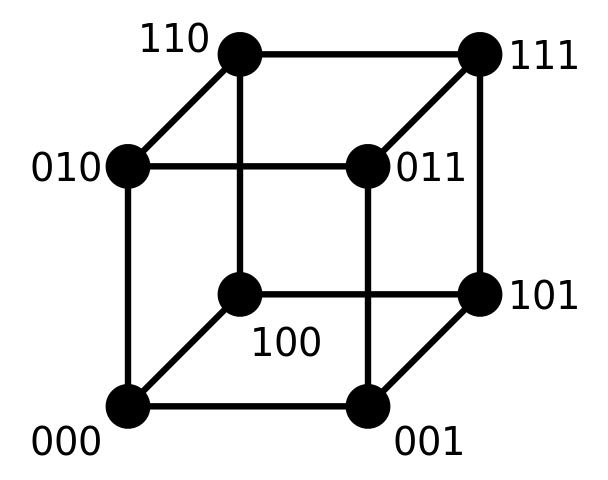
\includegraphics[width = 0.3\columnwidth]{Chaptersub/media/Hamming.png}
\caption{a Boolean cube $\cB = \{0,1\}^3$ \textcopyright\xspace \cite{pict}}
\label{fig.ham}
\end{figure}

We discuss why enlarging $\ee{f}$ is not a trivial feat. We build a bipartite graph $G:=(\cB \cup S_n, E)$. An edge $e$ of $E$ connects a vertex $v \in \cB$ to a permutation $\pi \in S_n$ if  $v \in V(\pi)$. Then, a minimal cover is a subset $S_n'$  of  $S_n$ such that: i) each vertex of $\cB$ is incident to at least one permutation in $S_n'$; ii) each permutation in $S_n'$ is incident to a vertex of $\cB$ that no other permutation in  $S_n'$ is incident to. As $|\cB| = 2^n$ and $|S_n|=n!$, the size of such a graph is not polynomial in $n$. We need additional information in order to enlarge $\ee{f}$ efficiently.


We relax the submodular maximization problem \eqref{eq.milp} through a polyhedral outer approximation $\cP$ of $\hyp_{\cB}(f)$. Let $X$ be the orthogonal projection of $\cP$ on $x$-space. We remark that, within a branch-and-cut algorithm, $X$ might be within a low-dimensional face of $\bar{\cB}$. Let $\relx{z}:=(\relx{x}, \relx{t})$ be an optimal basic feasible solution to the LP relaxation $\max_{(x,t) \in \cP} t$, which corresponds to a vertex of $\cP$. We assume that $\relx{x} \notin \cB$, otherwise, $\relx{x}$ is already an optimal solution to \eqref{eq.milp}.


As $\relx{z}$ is the point that we want to separate from $\hyp_{\cB}(f)$, we follow the method presented in \Cref{sec.premic} to construct an  intersection cut. According to \cite{conforti1984submodular,gomory1969some},  we can use a feasible basis of the LP relaxation to create a simplicial cone $\cR$. This cone $\cR$ can be easily obtained from the simplex tableau associated with the chosen basis.  In our case,  we select  the optimal basis defining $\relx{z}$ so that $\relx{z}$ is the apex of the corresponding cone $\cR$. Moreover, we use $\ee{f}$ as  $\hyp_{\cB}(f)$-free set. To determine whether the linear inequality \eqref{eq.ic} separates $\relx{z}$ from $\hyp_{\cB}(f)$, we need to verify whether $\relx{z} \in \inter(\ee{f})$.


The polyhedral outer approximation $\cP$ gives rise to a piece-wise linear concave overestimating function of $f$ over $X$: $\bar{f}(x) := \max_{(x,t) \in \cP} t$,
such that $\max_{(x,t) \in \cP} t = \max_{x \in X}\bar{f}(x)$. This implies that $\relx{t} = \bar{f}(\relx{x})$. We then have the following observation.  


\begin{proposition}
\label{prop.in}
Assume that $f$ is not affine over $X$. If $\relx{x} \in \relint(X)$, then $\bar{f}(\relx{x}) > \bsF_{f}(\relx{x})$, \ie $(\relx{x}, \bar{f}(\relx{x})) \in \inter(\ee{f})$.
\end{proposition}
\begin{proof}
As $\bar{f}$ is concave overestimator of $f$ over $X$ and $\bsF_{f}$ is convex  underestimator of $f$ over $X$, $\bar{f} \ge \bsF_{f}$ over $X$.  Suppose, to aim at a contradiction, that  $\bar{f}(\relx{x}) = \bsF_{f}(\relx{x})$. Define a concave function $g:= \bar{f} - \bsF_{f}$, then for all $x \in X$, $g(x) \ge 0$, and $g(\relx{x}) = 0$. By its concavity, there exists  an affine overestimating function $a$ of  $g$, such that $g(\relx{x}) = a(\relx{x}) = 0$, and, for all $x \in X$, $0 \le  g(x) \le a(x)$. As $\relx{x} \in \relint(X)$, the affinity of $a$  implies that $a = g = 0$ over $X$, \ie $\bar{f}= \bsF_{f}$ over $X$. So $f$ is concave and convex over $X$ and thus affine over $X$, which is a contradiction.
\end{proof}

The measure of the relative boundary $ \relbd(X)$ is zero, so we can assume that a mild \textit{relative interior condition} that $\relx{x} \in \relint(X)$ holds with probability one. Under this assumption,  the relaxation point  $\relx{z} = (\relx{x}, \bar{f}(\relx{x}))$ is  in the relative interior of the extended envelope epigraph with probability one. This implies that the linear inequality \eqref{eq.ic} separates $\relx{z}$ from $\hyp_{\cB}(f)$ with probability one. In  \Cref{sec.cresult}, we will empirically evaluate the effectiveness of these intersection cuts for various submodular maximization problems.
  
Throughout the rest of this chapter, we will encounter multiple nonconvex optimization problems. W.l.o.g., we will consider the simplicial cone defined by the simplex tableau associated with an optimal feasible basis of their LP relaxations. Such  simplicial cones are commonly employed in computational implementations. For the sake of brevity, we refer to such cones as \emph{optimal tableau cones}.
 
 \subsubsection{Extensions to SS functions}
\label{sec.ss}


This section considers Boolean-hypograph and  Boolean-superlevel sets for an SS function $f:=f_1 - f_2$, where $f_1$ and $f_2$ are two submodular functions. We extend our previous results on the Boolean-hypograph set of submodular functions; thus one can generate intersection cuts for a larger family of discrete nonconvex sets.

More specifically, we consider the following nonconvex set
\begin{equation}
    \label{eq.cs}
	 \cS := \{(x, t) \in \cB \times \bR: f(x)  \ge \ell t\},
\end{equation}
with $\ell \in  \{ 0, 1\}$. Given a relaxation point $(\relx{x}, \relx{t}) \notin \cS$,
we want to find cutting planes separating this point from $\cS$.


Let $\bsF_{f_1}  := \max_{s \in \ep{f_1}} sx$ and $\bsF_{f_2}  := \max_{s \in \ep{f_2}} sx$ be extended envelopes of $f_1, f_2$, respectively. As $\bsF_{f_1} $ (resp. $\bsF_{f_2} $) is a convex extension of $f_1$ (resp. $f_2$),  we have that $\cS = \{(x, t) \in \cB \times \bR: \bsF_{f_1} (x) - \bsF_{f_2} (x)  \ge \ell t\}.$ By relaxing $\cB$ to $\bR^n$,  a (nonconvex) continuous outer approximation of $\cS$ is
\begin{equation}
    \label{eq.csb}
	 \bar{\cS} := \{(x, t) \in \bR^n \times \bR: \bsF_{f_1} (x) - \bsF_{f_2} (x)  \ge \ell t\}.
\end{equation}
Moreover, for all $x \in \cB$, $(x,t) \in  \bar{\cS}$ if and only if $(x,t) \in  \cS$.

\textbf{Special cases. } When $ \ell = 1$, $\cS$ is the Boolean-hypograph of the SS function $f$; when $ \ell = 0$,  $\cS$ is the 0-superlevel set  of the SS function $f$ over the Boolean hypercube. Setting $f_2 = 0$ and $ \ell = 1 $, the set $\cS$  becomes the hypograph
$
    \{(x, t) \in \cB \times \bR: f_1(x) \ge t \},
$
which is studied in the previous section. Setting $f_1 = 0$, the relaxed set $\bar{\cS}$ becomes
$
    \{(x, t) \in \cB \times \bR: \bsF_{f_2} (x) \le -\ell t\}.
$
Let $(\relx{x}, \relx{t}) \notin \bar{\cS}$. Since $\bsF_{f_2} (x) \ge \gamma^\ast x$ and $\bsF_{f_2} (\relx{x}) = \gamma^\ast \relx{x}$  for any $\gamma^\ast \in \partial{\bsF_{f_2} }(\relx{x})$, then the simple outer approximation cut $ \gamma^\ast x \le -\ell t$ is a valid inequality for $\bar{\cS}$ (hence for $\cS$).







In general, we should separate intersection cuts specifically for SS functions. Let $\gamma^\ast \in \partial{\bsF_{f_2} }(\relx{x})$ be a solution to \eqref{eq.sep2} associated with $f_2$, and we define the  set
\begin{equation}
\label{eq.c}
	 \cC_{\relx{x}} := \{(x, t) \in \bR^n \times \bR:  \bsF_{f_1} (x) - \gamma^\ast x   \le\ell t\}.
\end{equation}
 
 The following proposition characterizes $\cS$-free sets for Eq.~\eqref{eq.csb}.
\begin{proposition}
\label{prop.dsfree}
The set $\cC_{\relx{x}}$ in \eqref{eq.c} is an $\cS$-free set. Moreover, if $(\relx{x}, \relx{t}) \notin \bar{\cS}$, then $\cC_{\relx{x}}$ does not contain $\relx{x}$ in its interior.
\end{proposition}
\begin{proof}
We first prove that $\cC_{\relx{x}}$ is $\bar{\cS}$-free. By definition, $\gamma^\ast x \le \bsF_{f_2} (x)$, which implies that $ \bsF_{f_1} (x) - \gamma^\ast x  \ge \bsF_{f_1} (x) - \bsF_{f_2} (x)  $. Therefore, for $(x,t) \in \inter(\cC_{\relx{x}})$, we have that $\ell t >   \bsF_{f_1} (x) - \gamma^\ast x  \ge \bsF_{f_1} (x) - \bsF_{f_2} (x) $, which implies that $(x,t) \notin \bar{\cS}$. Hence, $\inter(\cC_{\relx{x}}) \cap \bar{\cS} = \varnothing$. Additionally, $\cC_{\relx{x}}$ is convex. These two facts imply that $\cC_{\relx{x}}$ is $\bar{\cS}$-free. Since $\cS \subseteq \bar{\cS}$, $\cC_{\relx{x}}$ is also an $\cS$-free set. Next, assume that $(\relx{x}, \relx{t}) \notin \bar{\cS}$, then $ \ell \relx{t} >  \bsF_{f_1} (\relx{x}) - \bsF_{f_2} (\relx{x}) \le   \bsF_{f_1} (\relx{x}) - \gamma^\ast\relx{x} $, so $(\relx{x},\relx{t}) \in \inter(\cC_{\relx{x}})$.
\end{proof}

In \cite{munoz2020maximal,serrano2019,xusignomial}, the authors study  the sub/superlevel sets of some DC functions.
Their construction of $\cS$-free sets relies on a common \textit{reverse-linearization technique}: reverse the set $\cS$ by changing the sign of its defining inequality, and linearize one  convex function.

In  our case, $f$ is an SS function, so we first need to extend the submodular and supermodular components of $f$. After the extension, we obtain a DC function. We can then  apply the reverse-linearization technique to its continuous extension.

\section{Convex envelopes of supermodular functions}
\label{sec.conenvesuper}

We know overestimators for submodular functions in \Cref{sec.concaveover}. However, we do not know their concave envelopes. In this section, w.l.o.g., we consider supermodular functions and their convex envelopes.
We present a general characterization of convex envelopes of supermodular functions.


Let $f:Q \to \bR$ be a supermodular function, where $Q:=\{0,1\}^h$. We can use a bit representation to denote Boolean points in $Q$. For example, $10$ denotes the point $w$ that $w_1 = 1$ and $w_2 = 0$. For an affine function $a\cdot w + b$, its \emph{supporting points} are the Boolean points in $Q$ where $a\cdot w + b$ equals $f(w)$.

\begin{lemma}
\label{lem.simplex}
Every facet of $f$ has $h+1$ affinely independent supporting points in $Q$.
\end{lemma}
\begin{proof}[Proof of \Cref{lem.homo}]
Given $z \in \dom(f)$, $f(\rho z)= \rho^d f(z) $ is a real number for any  $\rho \in \bR_{++}$, so $\inter(\dom(f))$ is a cone.
Suppose that $f$ is positive homogeneous of degree 1. For any $z \in \dom(f)$,
$
	\lin{f}{\breve{z}}(z) = f(\breve{z}) + \nabla  {f}(\breve{z}) \cdot (z - \breve{z}) =  \nabla  {f}(\breve{z}) \cdot z,
$
where  the second equation follows from Euler's homogeneous function theorem: $f(\breve{z}) = \nabla {f}(\breve{z}) \cdot \breve{z}$. For any \( z = \rho \breve{z}\) with \(\rho \in \bR_{++}\),
$
	\lin{f}{\breve{z}}(z)  = \nabla  {f}(\breve{z})\cdot \rho \breve{z} = \rho  \lin{f}{\breve{z}}(\breve{z}) =\rho f( \breve{z}) = f(\rho \breve{z}),
$
where the first and second equations follow from the previous result, the third follows from that $\lin{f}{\breve{z}}$ has the same value as $f$ at $\breve{z}$, and the last equation follows from the homogeneity.
\end{proof}
\begin{proof}
        We note that any hyperplane in $\bR^{h+1}$ is uniquely determined by $h+1$ affinely independent points. By definition, an affine underestimator  $a\cdot w + b$ of $f$ is a facet if and only if $a\cdot w + b \le t$ is a facet of the epigraph $\epi_{Q}(f)$.  Then, the affine underestimator  is a facet, if and only if, there exists $h+1$ affinely independent points $\{(w^i, t^i)\}_{i \in [h+1]} \subseteq \epi_{Q}(f) \subseteq \bR^{h+1}$  such that for all $i \in [h+1]$, $a\cdot w^i + b =  t^i$.  Moreover, $t^i$ must equal $f(w^i)$, otherwise $a\cdot w^i + b =  t^i < f(w^i)$, which implies that $a\cdot w + b \le t$ does not underestimate $f$ at $w^i$. Therefore, $w^i$ is the supporting point of $a\cdot w + b$. Note that $\{(w^i, t^i)\}$ are affinely independent, if only if, $\{w^i\}_{i \in [h+1]}$ are affinely independent. 
\end{proof}

We can enumerate all possible subsets of $h+1$ affinely independent points of  $Q$. Each such subset $S \deq  \{w^1,\dots,w^{h+1}\}$ determines an function over $\bR^h$ via the following affine combination:
\begin{equation*}
    f_S(w) \deq \{\sum_{j \in [h+1]}\lambda_j f(w^j) : \exists \lambda \in \bR^{h+1} \, \sum_{j \in [h+1]}\lambda_j=1 \land \sum_{j \in [h+1]}\lambda_j w^j = w\}.
\end{equation*} 
Due to the affine independence of $S$, the Barycentric coordinate $\lambda$ for each $w$ in the above affine combination is unique.  We can consider $f_S$ as a single-valued affine function and call it the \emph{supported function} of $S$. Since,  for all $w \in S$, $f_S(w)=f(w)$, solving the linear system $a \cdot w + b = f(w) (w \in S)$, we can compute $a,b$ defining $f_S$.
If the supported function $f_S$ underestimates $f$, we call the subset $S$ \emph{facet-inducing}. 

Assuming we have a collection of facets of $f$, we then determine whether these facets define the convex envelope of $f$. We recall that the convex hull of $h+1$ affinely independent points is called an  \emph{$h$-simplex}.
A finite collection of $h$-simplices $\{P_k\}_k$ is called a \emph{triangulation} of the unit cube $\cU$, if the following conditions hold: (i) $\bigcup_{k} P_k = \cU$, (ii)  $P_k \cap P_{k'}$ is empty or a face of both $P_k \cap P_{k'}$ for all $k, k'$, (iii) the vertices of $P_k$ are contained in $Q$ for all $k$.


\begin{proposition}\label{prop.triangle}
Let $\{S_k\}_{k}$ be a collection of facet-inducing subsets of $Q$. For each $k$, let $f_{S_k}$ be the supported function induced by $S_k$, and let $P_k:= \conv(S_k)$ be the simplex spanned by $S_k$. If  $\{P_k\}_k$ is  a triangulation of $\cU$, then $\conve_{\cQ}(f)(w) = \max_{k} f_{S_k}(w)$ for all $w \in \cU$.
\end{proposition}
\begin{proof}
Since $\bigcup_{k} P_k = \cU$, for any $w \in Q$, there exists $P_k$ such that $w \in P_k$. Since the vertices $S_k$ of $P_k$ are contained in $Q$, $w$ must be in $S_k$. Therefore, $f_{S_k}(w) = f(w)$.
This implies that $f(w) = \max_{k} f_{S_k}(w)$ for all $w \in Q$, \ie $ \max_{k} f_{S_k}$ is an exact convex underestimator. Suppose, to aim at a contradiction, that there exists another convex underestimator $f'$ of $f$ such that $f'(w) = f(w)$ for all $w \in Q$, and $f'(w') > \max_{k} f_{S_k}(w')$ for some $w' \in \cU$.  Again, since $\bigcup_{k} P_k = \cU$, there exists $P_k$ such that $w' \in P_k$, \ie $w' \in \conv(S_k)$. Let $S_k = \{w^1,\dots,w^{h+1}\}$. It follows from $w' \in \conv(S_k)$ that there exists $\lambda \in [0,1]^{h+1}$ such that $\sum_{j \in [h+1]}\lambda_j=1,\sum_{j \in [h+1]}\lambda_j w^j = w'$. Note that $S_k$ induces the supported function $f_{S_k}$, which has supporting points $S_k$. This implies that $f_{S_k}(w') = \sum_{j \in [h+1]}\lambda_j f_{S_k}(w^j) = \sum_{j \in [h+1]}\lambda_j f(w^j)$. It follows from the convexity of $f'$ that $f'(w') \le \sum_{j \in [h+1]}\lambda_j f'(w^j) = \sum_{j \in [h+1]}\lambda_j f(w^j) \le f_{S_k}(w') \le  \max_{k} f_{S_k}(w')$, which leads to a contradiction. Therefore, $ \max_{k} f_{S_k}$ is the convex envelope of $f$ over $\cQ$.
\end{proof}

The collection $\{S_k\}_{k}$ is called  \emph{envelope-inducing} family in $Q$, if the presupposition ``$\{P_k\}_k$ is  a triangulation'' in  \Cref{prop.triangle} is satisfied.


